% SmartSense Monitoring - HardwareX article
% Built on the official HardwareX article template (Version 2, June 2021).
% Template instructions (italic text) have been removed as required before submission.
\documentclass[11pt, letterpaper]{article}
\usepackage[utf8]{inputenc}
\usepackage[margin=1.5cm]{geometry}
\usepackage{titlesec}
\usepackage{tabu}
\usepackage{enumitem}
\usepackage{amssymb}
\usepackage{xcolor}
\usepackage{graphicx}
\graphicspath{{../figuras/}}
\usepackage{placeins}

\usepackage{lmodern}
\usepackage{hyperref}
\hypersetup{colorlinks=true, linkcolor=blue, filecolor=magenta, urlcolor=blue}
\urlstyle{same}

\titleformat{\section}[block]{\hspace{1em}\bfseries}{\thesection.}{0.5em}{}
\titleformat{\subsection}[block]{\hspace{1em}}{\thesubsection}{0.5em}{}

\setlength{\parindent}{0pt}
\setlength{\parskip}{10pt}

\begin{document}
\begin{flushleft}

\textbf{Article title}\\
SmartSense Monitoring: an open-source wireless PT100 node and gateway for long-term surface-temperature monitoring of industrial equipment

\textbf{Authors}\\
Jesus Andre Bojaca Lopez, David Santiago Puentes Cardenas*, Jhon Edwin Vera, Sergio Francisco Mora Martinez

\textbf{Affiliations}\\
Electronic Engineering Program, Faculty of Engineering, Universidad ECCI, Bogota D.C., Colombia

\textbf{Corresponding author's email address and Twitter handle}\\
davids.puentesc@ecci.edu.co

\textbf{Abstract}\\
SmartSense Monitoring is an open-source wireless system for measuring and logging the surface temperature of industrial equipment. Each battery-powered node combines a Seeed Studio XIAO ESP32-C6 microcontroller, a three-wire PT100 probe, a MAX31865 RTD front-end and an Ebyte E220 LoRa radio at 433~MHz. A gateway based on a second ESP32-C6 with an integrated touch display receives the frames, stores a per-sensor daily history on a microSD card (with LittleFS as a fallback) and serves a local web dashboard over Wi-Fi, requiring no cloud service or permanent Internet connection. Unlike a handheld spot measurement, the system preserves the continuous 24-hour thermal behaviour of each machine, enabling the detection of trends and anomalies. Over a 32-day pilot deployment with three nodes (51{,}338 samples), the LoRa link availability exceeded 97\% once scheduled plant stoppages were excluded, and the continuous history revealed a temperature rise on a suction-fan motor later associated with a bearing anomaly. All design files, firmware and the bill of materials are released under open-source licenses.

\textbf{Keywords}\\
Open-source hardware; LoRa; PT100; RTD; MAX31865; ESP32-C6; industrial temperature monitoring; predictive maintenance

\newpage
\textbf{Specifications table}\\
\vskip 0.2cm
\tabulinesep=1ex
\begin{tabu} to \linewidth {|X|X[3,l]|}
\hline \textbf{Hardware name} & SmartSense Monitoring \\
\hline \textbf{Subject area} &
  \begin{itemize}[noitemsep, topsep=0pt]
  \item Engineering and material science
  \item Educational tools and open source alternatives to existing infrastructure
  \end{itemize} \\
\hline \textbf{Hardware type} &
  \begin{itemize}[noitemsep, topsep=0pt]
  \item Measuring physical properties and in-lab sensors
  \item Field measurements and sensors
  \item Electrical engineering and computer science
  \end{itemize} \\
\hline \textbf{Closest commercial analog} & Industrial wireless RTD/condition-monitoring loggers such as the Advantech WISE-2410 and commercial PT100 wireless data loggers. \\
\hline \textbf{Open source license} & Hardware: CERN-OHL-S v2. Firmware and software: MIT License. Documentation: CC-BY 4.0. \\
\hline \textbf{Cost of hardware} & Approximately 170~USD for three nodes and one gateway (see Bill of materials). Approximately 35~USD per additional node. \\
\hline \textbf{Source file repository} & Available in the article (to be deposited at Zenodo with a DOI upon acceptance). \\
\hline
\end{tabu}
\end{flushleft}

\newpage
\section{Hardware in context}

Continuous temperature monitoring of motors and other industrial equipment helps identify conditions associated with friction, overload, poor ventilation or mechanical degradation. In a manual inspection, an operator obtains only the value at the instant of measurement; if that value is not systematically recorded, the thermal evolution of the equipment cannot be reconstructed or related to its operating and stop cycles.

Wireless sensor networks distribute measurement points without installing communication cabling at each location. For low-data-rate applications, LoRa provides a long-range, low-power alternative suited to battery-powered nodes. Several open-source LoRa temperature nodes have been published, but they typically target ambient or DHT-class humidity/temperature sensors and rely on a cloud back-end. SmartSense Monitoring differs in three respects relevant to industrial surface monitoring: (i) it uses an industrial-grade three-wire PT100 with a MAX31865 front-end rather than a low-cost ambient sensor; (ii) it stores a per-sensor daily history locally and serves the dashboard from the gateway itself, so it operates without Internet; and (iii) the design targets replication and customization, releasing the schematics, firmware and bill of materials under open-source licenses.

A PT100 RTD was chosen over a digital sensor such as the DS18B20 for several reasons: the PT100 is the industrial standard (IEC~60751) with excellent long-term stability and low drift; its resistive nature allows precise analog conditioning through the MAX31865, a purpose-built RTD-to-digital converter for two-, three- and four-wire PT100 with lead-resistance compensation; it offers a far wider range ($-200$ to $850~^{\circ}$C) than the DS18B20 ($-55$ to $125~^{\circ}$C), suitable for industrial surfaces that may exceed the digital sensor's limit; and it is available in surface-mount and magnetic probe forms appropriate for mounting on motors.

Compared with proprietary industrial loggers such as the Advantech WISE-2410, SmartSense Monitoring trades integrated vibration sensing for a lower cost, full openness and local-first operation, making it suitable for pilot plants and educational settings where flexibility and reproducibility matter more than a turnkey platform.

\section{Hardware description}

SmartSense Monitoring consists of one or more battery-powered sensor nodes and a gateway/visualizer. Each node acquires the surface temperature of a machine with a magnetic PT100 probe and a MAX31865 RTD front-end, estimates its battery state, and transmits the reading over a 433~MHz LoRa link before entering deep sleep. The gateway receives the frames, identifies each node by its MAC address, applies a configurable offset, stores the samples locally and presents them on an integrated touch display and a Wi-Fi web dashboard.

\begin{itemize}
\item[$\bullet$] It provides continuous, unattended surface-temperature logging of industrial equipment at a fraction of the cost of commercial wireless RTD loggers, using widely available modules.
\item[$\bullet$] It operates fully offline: the gateway serves its own dashboard over a local Wi-Fi access point, so no cloud account or Internet connection is required.
\item[$\bullet$] It preserves a per-sensor daily history, enabling the study of thermal trends, transients and machine on/off cycles that a spot measurement cannot capture.
\item[$\bullet$] It is a modular basis for further work: additional nodes, alternative RTD probes, or extra variables (e.g. current, vibration) can be integrated by reusing the node design.
\item[$\bullet$] It is suitable as a teaching platform for wireless sensor networks, RTD signal conditioning, embedded firmware and edge data handling, since every layer is open and documented.
\end{itemize}

\section*{\textit{Design files}}

The complete design files (KiCad schematics, firmware, bill of materials) are provided with the article and will be deposited in an open repository (Zenodo) with a DOI upon acceptance. The schematics are provided in editable KiCad format; the firmware source is fully included and commented.

\section{Design files summary}
\vskip 0.1cm
\tabulinesep=1ex
\begin{tabu} to \linewidth {|X|X|X[1.5,1]|X[1.5,1]|}
\hline
\textbf{Design filename} & \textbf{File type} & \textbf{Open source license} & \textbf{Location of the file} \\\hline
Node schematic (nodo\_sensor) & KiCad schematic (.kicad\_sch) + PDF/SVG & CERN-OHL-S v2 & Available with the article \\\hline
Gateway schematic (gateway) & KiCad schematic (.kicad\_sch) + PDF/SVG & CERN-OHL-S v2 & Available with the article \\\hline
smartsense.kicad\_sym & KiCad symbol library & CERN-OHL-S v2 & Available with the article \\\hline
Node firmware (Nodo\_Lora) & Arduino C++ (.ino) & MIT & Available with the article \\\hline
Gateway firmware (maestro\_Lora\_pantalla) & Arduino C++ (.ino) + web assets & MIT & Available with the article \\\hline
Bill of materials (BOM.csv) & CSV spreadsheet & CC-BY 4.0 & Available with the article \\\hline
Enclosure (node/gateway) & 3D model (STL + source CAD) & CERN-OHL-S v2 & To be added \\\hline
\end{tabu}

\vskip 0.3cm
The node and gateway schematics document every external connection (SPI to the MAX31865, UART to the E220, switched sensor power, and the battery divider), verified against the firmware. The firmware files contain the node acquisition/transmission loop and the gateway reception, storage and dashboard logic. The bill of materials lists every purchasable component. The enclosure design files (PLA, 3D-printed) will be added to the repository.

\section*{\textit{Bill of materials}}

Costs are given in Colombian pesos (COP) with an approximate US dollar (USD) equivalent, based on the actual procurement prices of the project. The table below covers three nodes and one gateway. Prices vary by supplier and availability.

\section{Bill of materials summary}
\vskip 0.2cm
\tabulinesep=1ex
\begin{tabu} to \linewidth {|X[1.1,1]|X|X[0.6,1]|X[0.9,1]|X[0.9,1]|X|X[1.1,1]|}
\hline
\textbf{Designator} & \textbf{Component} & \textbf{Number} & \textbf{Cost per unit (COP)} & \textbf{Total (COP)} & \textbf{Source of materials} & \textbf{Material type} \\\hline
U1 & Seeed Studio XIAO ESP32-C6 (node) & 3 & 30{,}000 & 90{,}000 & \href{https://www.seeedstudio.com/}{seeedstudio.com} & Semiconductor \\\hline
U2 & ESP32-C6 Touch LCD 1.47 board (gateway) & 1 & 90{,}000 & 90{,}000 & Local distributor & Semiconductor \\\hline
U3 & Ebyte E220-433 LoRa module + antenna & 4 & 30{,}000 & 120{,}000 & \href{https://ebyteiot.com/}{ebyteiot.com} & Semiconductor \\\hline
RT1 & Magnetic three-wire PT100 probe & 3 & 30{,}000 & 90{,}000 & Local distributor & Metal \\\hline
U4 & MAX31865 RTD front-end module & 3 & 14{,}000 & 42{,}000 & \href{https://www.sigmaelectronica.net/}{sigmaelectronica.net} & Semiconductor \\\hline
BT1 & LiPo battery 3.7~V 2000~mAh & 3 & 30{,}000 & 90{,}000 & \href{https://www.didacticaselectronicas.com/}{didacticaselectronicas.com} & Other \\\hline
U5 & LiPo charge/protection module (TP4056 or equiv.) & 3 & 5{,}000 & 15{,}000 & Local distributor & Semiconductor \\\hline
R1 & Resistor 344.8~k$\Omega$ (battery divider) & 3 & -- & -- & Local distributor & Other \\\hline
R2 & Resistor 994.3~k$\Omega$ (battery divider) & 3 & -- & -- & Local distributor & Other \\\hline
MEC1 & 3D-printed PLA enclosure & 4 & 10{,}000 & 40{,}000 & Self-printed & Polymer \\\hline
W1 & Wires, connectors, headers, hardware, adhesives & 1 & 50{,}000 & 50{,}000 & Local distributor & Other \\\hline
\end{tabu}\\
\vskip 0.2cm
Approximate total: 627{,}000~COP ($\approx$ 155~USD) plus a contingency allowance. The battery-divider resistors are drawn from a general parts kit and are accounted for in the wiring line item.

\section{Build instructions}

The following steps describe the construction of one sensor node and the gateway. Refer to the node and gateway schematics (Design files) and to the Bill of materials for component designators.

\textbf{Sensor node}
\begin{enumerate}[noitemsep]
\item Solder the MAX31865 module in three-wire mode (bridge the 2/3-wire jumper), and connect the PT100 leads: the two leads from the same probe end to F+ and RTD+, and the remaining lead to RTD-, bridged to F-.
\item Wire the MAX31865 SPI bus to the XIAO ESP32-C6: CLK\,$\rightarrow$\,D6 (GPIO16), SDO\,$\rightarrow$\,D5 (GPIO23), SDI\,$\rightarrow$\,D4 (GPIO22), CS\,$\rightarrow$\,D3 (GPIO21). Power the module VIN from D2 (GPIO2) so the firmware can switch it off during deep sleep.
\item Connect the E220 LoRa module by UART: E220 TXD\,$\rightarrow$\,D7 (GPIO17), RXD\,$\rightarrow$\,D8 (GPIO19), M0\,$\rightarrow$\,D10 (GPIO18), M1\,$\rightarrow$\,D9 (GPIO20); power VCC/GND from 3V3/GND.
\item Build the battery divider: VBAT\,--\,R1 (344.8~k$\Omega$)\,--\,A0 (GPIO0)\,--\,R2 (994.3~k$\Omega$)\,--\,GND. Connect the LiPo cell through the TP4056 charge/protection module to the XIAO battery pads.
\item Flash the node firmware (\texttt{Nodo\_Lora.ino}) with the Arduino IDE and the ESP32 board package. Install the Adafruit\_MAX31865 library. Set \texttt{RREF} to the measured reference resistance of your MAX31865 module (421.1~$\Omega$ in this build).
\item Fit the components in the 3D-printed PLA enclosure and attach the PT100 magnetically to the target surface.
\end{enumerate}

\textbf{Gateway}
\begin{enumerate}[noitemsep]
\item Connect the E220 module to the ESP32-C6 Touch LCD board: E220 TXD\,$\rightarrow$\,GPIO7, RXD\,$\rightarrow$\,GPIO8, and both M0 and M1 to GPIO9; power VCC/GND from 3V3/GND.
\item Optionally wire a critical-alarm output (LED, buzzer or relay driver) to GPIO16.
\item Flash the gateway firmware (\texttt{maestro\_Lora\_pantalla.ino}) and upload the web dashboard assets to the on-board storage (LittleFS). Insert a microSD card for the history.
\end{enumerate}

\textbf{Safety.} Use a fused LiPo cell with the TP4056 protection module and observe LiPo handling precautions. Ensure the PT100 and enclosure are rated for the surface temperature of the monitored equipment and mounted so they do not interfere with moving parts.

\begin{figure}[h]\centering
\begin{minipage}[b]{0.44\linewidth}\centering
  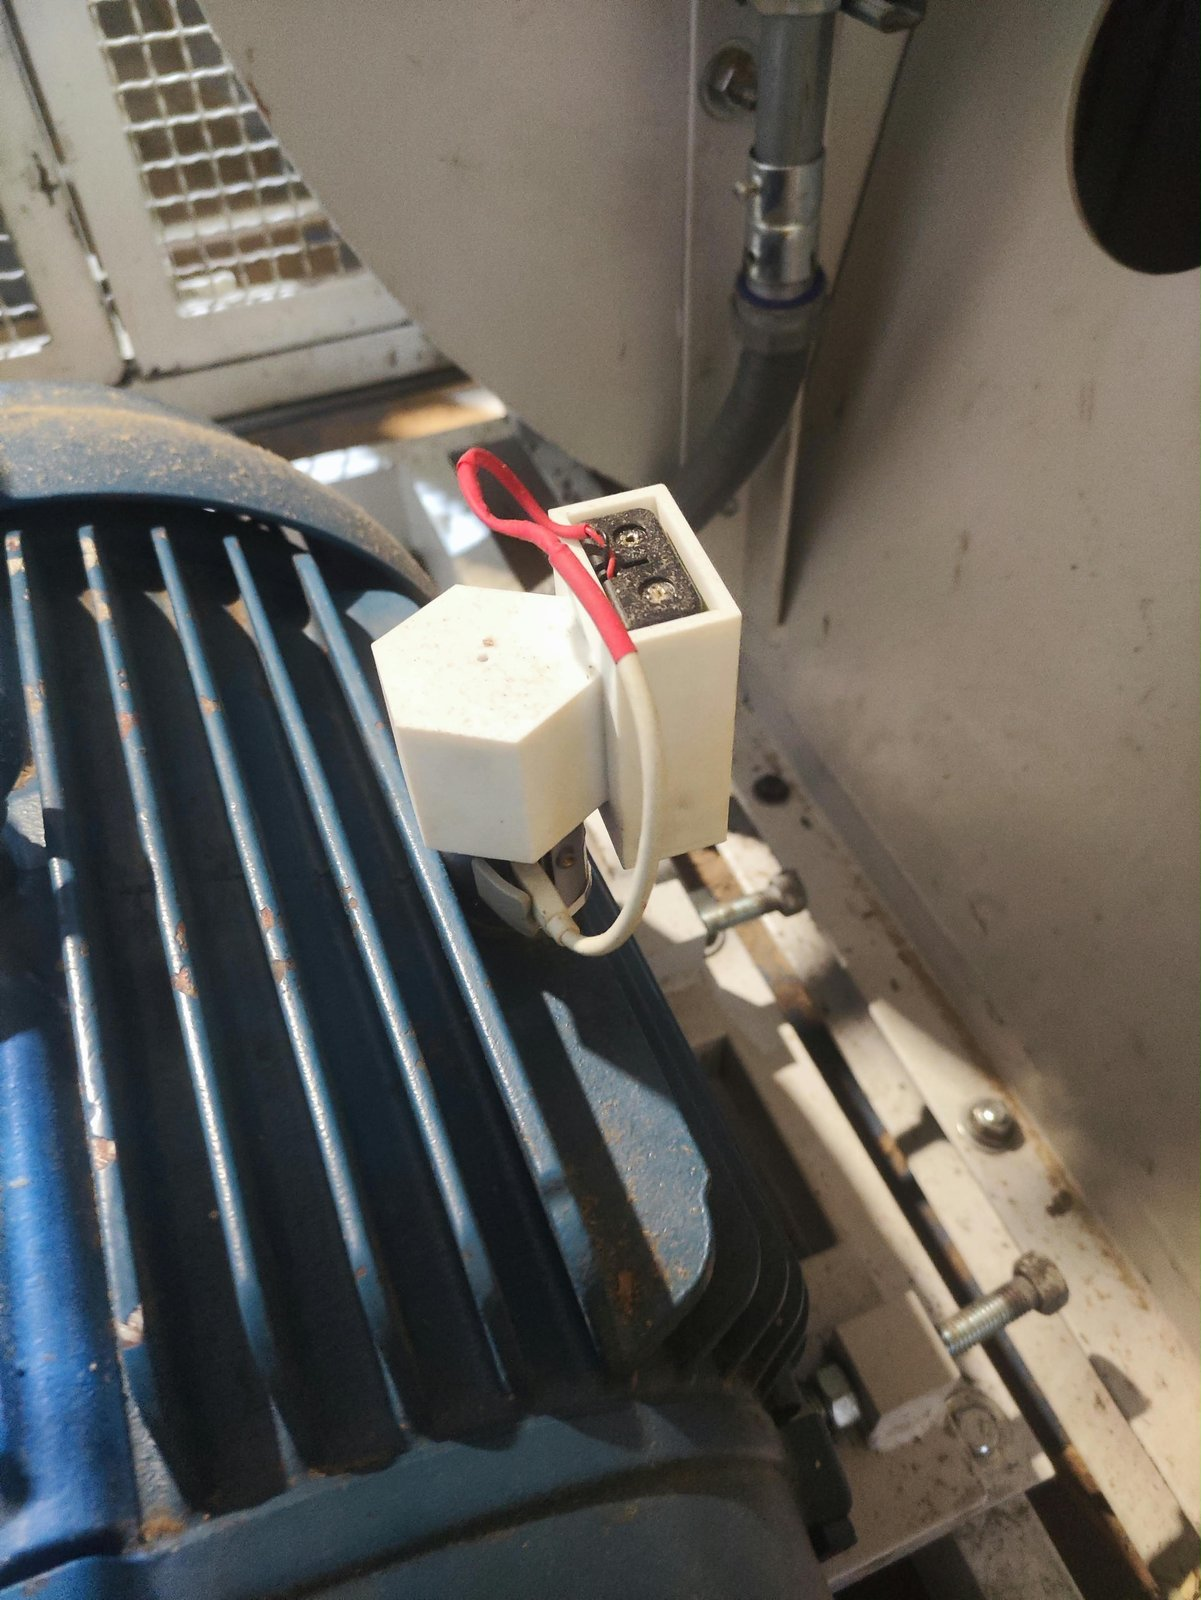
\includegraphics[height=5cm]{evidencias/nodo-instalado.jpg}
\end{minipage}\hfill
\begin{minipage}[b]{0.44\linewidth}\centering
  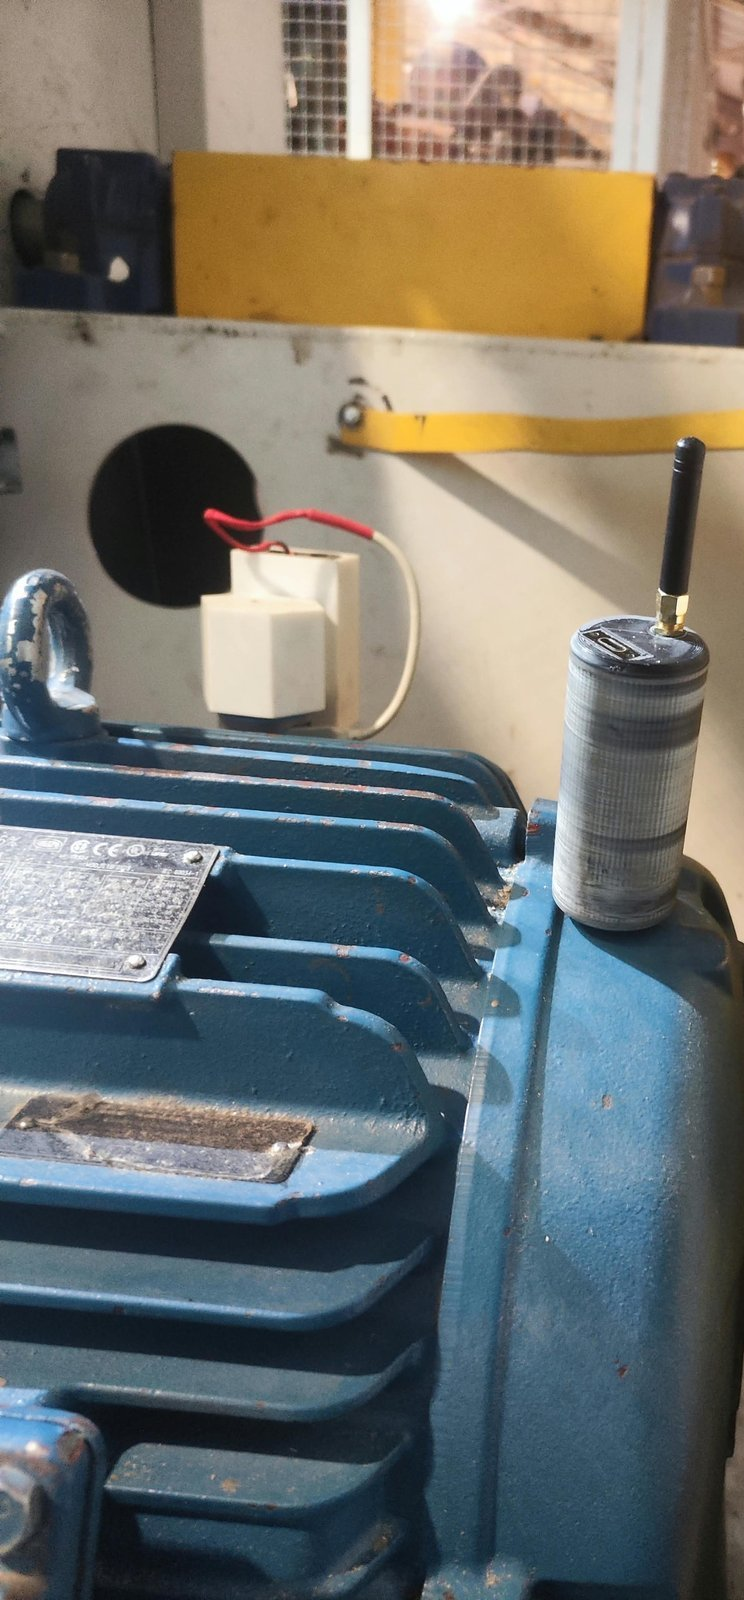
\includegraphics[height=5cm]{evidencias/nodo-antena-neutro.jpg}
\end{minipage}
\caption{Assembled sensor node mounted on a motor housing: the PT100 probe with the MAX31865 module (left) and the node enclosure with the LoRa antenna (right).}
\label{fig:node-photo}
\end{figure}

\section{Operation instructions}

\begin{enumerate}[noitemsep]
\item Power the gateway. It creates a Wi-Fi access point (\texttt{Sensores\_Temp}) and serves the dashboard at \texttt{http://192.168.4.1}.
\item Power each node. On first boot it transmits periodically (default configurable between 5 and 7200~s; 120~s in the pilot). The gateway registers each node by its MAC address.
\item In the dashboard, assign names to sensors, group them by machine, set the sampling interval, apply a per-node temperature offset, and configure warning and critical thresholds.
\item Monitor the live values (temperature, battery, connectivity) and consult the per-day 24-hour history, including minimum, maximum and average, and compare sensors of the same machine.
\item To analyse data off-line or export figures, download the per-sensor history; the accompanying software replica can bulk-import the exported CSV.
\end{enumerate}

\begin{figure}[h]\centering
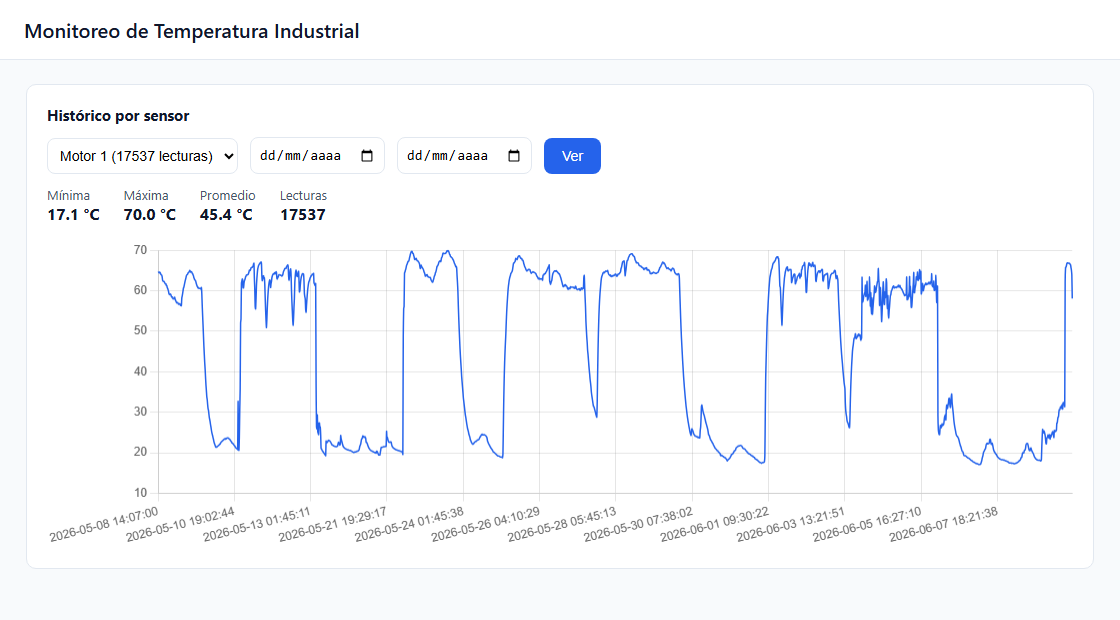
\includegraphics[width=\linewidth]{dashboard-neutro.png}
\caption{Local web dashboard: per-sensor temperature history over the deployment, with minimum, maximum and mean statistics. Shown here running on the open-source software replica with generic sensor labels.}
\label{fig:dashboard}
\end{figure}

\textbf{Safety.} The critical-alarm output is a supervisory aid, not a safety interlock; do not use it as the sole protection for equipment or personnel.

\section{Validation and characterization}

The system was validated in a pilot plant with three nodes over a 32-day deployment, producing 51{,}338 stored samples with a median sampling interval of 121~s.

\textbf{Availability.} Data outages were found to occur \emph{simultaneously} across all three nodes, with identical start times (Fig.~\ref{fig:cobertura}). This pattern indicates that the interruptions were periods with the gateway powered off (plant and power stoppages) rather than LoRa link failures, which would affect a single node at a time. Accordingly, Table~\ref{tab:avail} reports both the raw availability over the full deployment and the link availability computed over the active intervals only (i.e. excluding the documented gateway-off periods). The link availability exceeded 97\% for all three nodes.

\begin{table}[h]
\centering
\tabulinesep=1ex
\begin{tabu} to \linewidth {|X|X[c]|X[c]|X[c]|X[c]|X[c]|}
\hline
\textbf{Node} & \textbf{Samples} & \textbf{Raw avail.} & \textbf{Link avail.} & \textbf{Stoppages} & \textbf{Hours off} \\\hline
Node A & 17{,}537 & 76.0\% & 98.4\% & 66 & 176 \\\hline
Node B & 16{,}487 & 32.3\% & 98.3\% & 73 & 1154 \\\hline
Node C & 17{,}314 & 75.1\% & 97.8\% & 81 & 180 \\\hline
\end{tabu}
\caption{Availability per node. Link availability excludes gateway-off periods, identified by their simultaneity across nodes. Node B includes a prolonged $\sim$33-day stoppage.}
\label{tab:avail}
\end{table}

\textbf{Reception cadence and packet loss.} During active intervals the frame inter-arrival time was tightly concentrated around the 121~s median (Fig.~\ref{fig:intervalos}), confirming a stable reception cadence. Estimating losses from the arrival intervals (a gap of $k$ times the cycle implies $k-1$ missing frames), the packet loss during active operation was 3.5--4.7\% across the three nodes, i.e. a packet delivery ratio of 95--97\%.

\textbf{Representative 60-minute test.} A representative one-hour window with the three nodes active (Fig.~\ref{fig:prueba60}) illustrates a continuous test: at a 120~s cycle, 30 frames are expected per node in 60~min; 29, 30 and 30 were received (PDR 96.7\%, 100\%, 100\%). Temperature and PDR are captured in this window; battery is characterised separately (Fig.~\ref{fig:autonomia}) and recovery after a reset is 2.279~s. RSSI and SNR are not exposed by the current E220 firmware configuration, and end-to-end latency requires node--gateway clock synchronisation; both are declared as future work. The node frame now carries a sequence counter, enabling a fully instrumented sent-vs-received PDR in a repeated test.

\begin{figure}[h]\centering
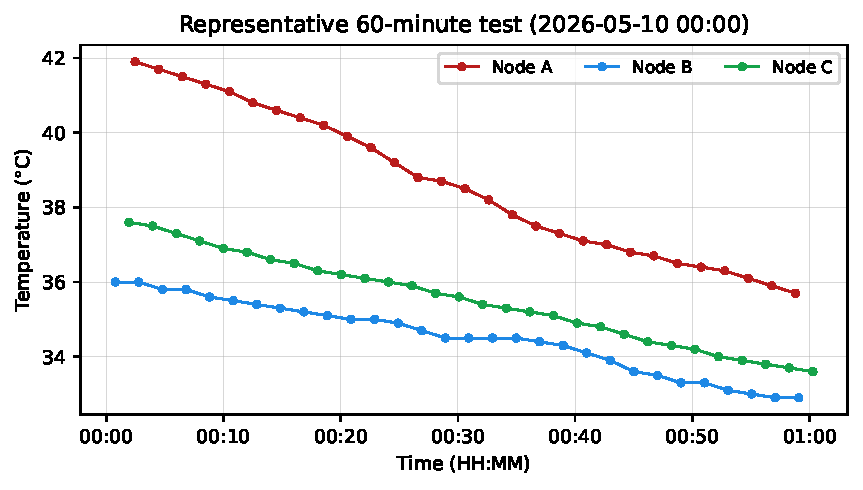
\includegraphics[width=0.9\linewidth]{prueba-60min.pdf}
\caption{Representative 60-minute window (three nodes active) showing temperature versus time during a night-time cool-down of the machines.}
\label{fig:prueba60}
\end{figure}

\textbf{Temperature agreement.} Five paired readings were taken simultaneously at the same surface point of the suction-fan motor, in the 65--71~$^{\circ}$C range, against a Fluke 62 MAX infrared thermometer (accuracy $\pm$1.5~$^{\circ}$C or $\pm$1.5\%, fixed 0.95 emissivity, used as a field reference without a current calibration certificate). The SmartSense readings agreed with the Fluke within $\pm$0.4~$^{\circ}$C (mean difference $\approx$0.1~$^{\circ}$C). Two caveats apply: the per-node offset was tuned using the same Fluke, and the Fluke's own accuracy ($\pm$1.5~$^{\circ}$C) exceeds the $\leq$1~$^{\circ}$C target. This therefore demonstrates that the compensation reproduces the reference, but is not an independent accuracy validation; a rigorous $\leq$1~$^{\circ}$C characterization over a wider range and across all three nodes would require a calibrated contact reference (thermocouple or reference RTD).

\textbf{Use case.} The continuous history captured a surface-temperature rise on a suction-fan motor, reaching a maximum of 70.0~$^\circ$C (Fig.~\ref{fig:serie}). The rising segments corresponded to periods when the machine stopped while the fan motor kept spinning unloaded; the pattern was later related to a bearing anomaly. This demonstrates the practical value of continuous logging over spot measurements.

\textbf{Recovery and temperature range.} After a node reset, the node boots, samples and transmits its first frame in about 2.279~s (measured from the firmware), well within one sampling cycle and far below any practical requirement. Across the three nodes, the recorded surface temperature spanned 15.3--70.0~$^{\circ}$C, with per-node mean values of 39.5--45.4~$^{\circ}$C.

\textbf{Battery autonomy.} A discharge test with a 1000~mAh cell (node in normal operation) showed the voltage dropping from 4.112~V to 4.089~V over 5 days (0.19~mV/h). Because the LiPo discharge is non-linear, autonomy was estimated two ways (Fig.~\ref{fig:autonomia}): a linear extrapolation gives a conservative lower bound of $\approx$177 days, whereas modelling the typical LiPo voltage--state-of-charge curve (calibrated to the measured points) gives $\approx$290--307 days ($\approx$10 months). The implied average current is 0.13--0.24~mA, consistent with the measured 1.9\% duty cycle (deep sleep $\approx$15~$\mu$A for 98.1\% of the time plus a 2.279~s active pulse). With the 2000~mAh battery of the prototype the autonomy would roughly double.

\begin{figure}[h]\centering
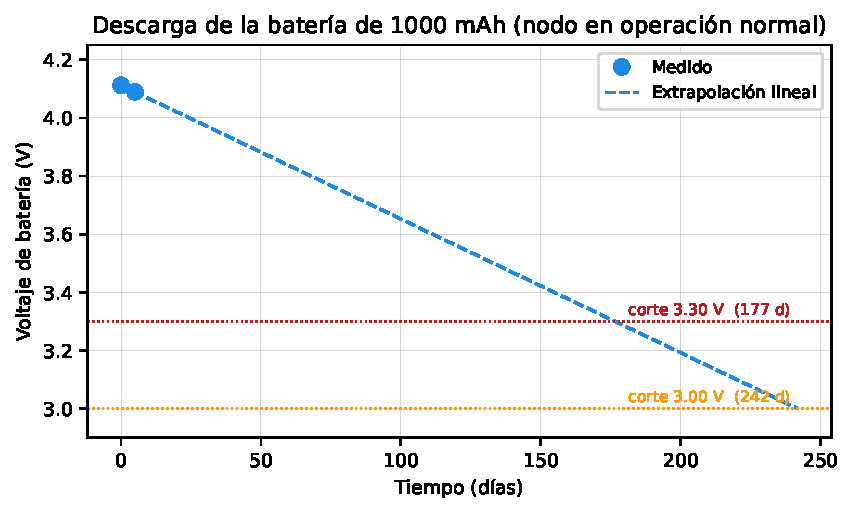
\includegraphics[width=0.9\linewidth]{autonomia-descarga.pdf}
\caption{Battery discharge test (1000~mAh cell): measured points, non-linear LiPo discharge model (voltage--state-of-charge curve) and a linear extrapolation as a conservative lower bound. The model estimates an autonomy of about 10 months.}
\label{fig:autonomia}
\end{figure}

\begin{figure}[h]\centering
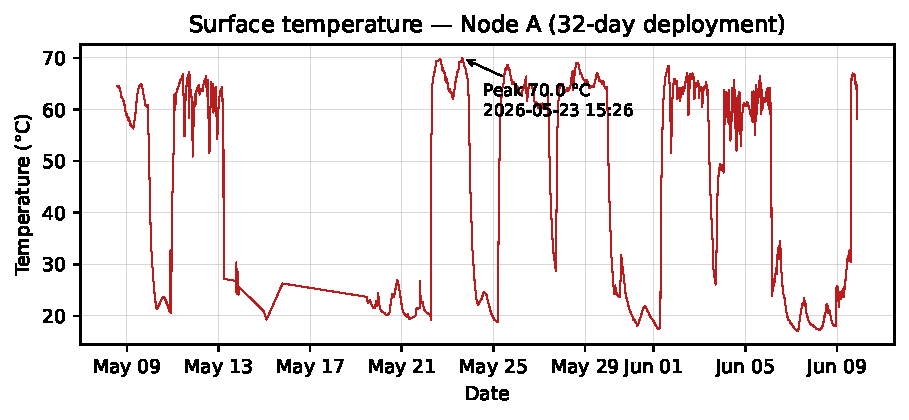
\includegraphics[width=0.9\linewidth]{val-serie-evento.pdf}
\caption{Surface temperature of one node over the 32-day deployment, showing the maximum associated with the suction-fan case.}
\label{fig:serie}
\end{figure}

\begin{figure}[h]\centering
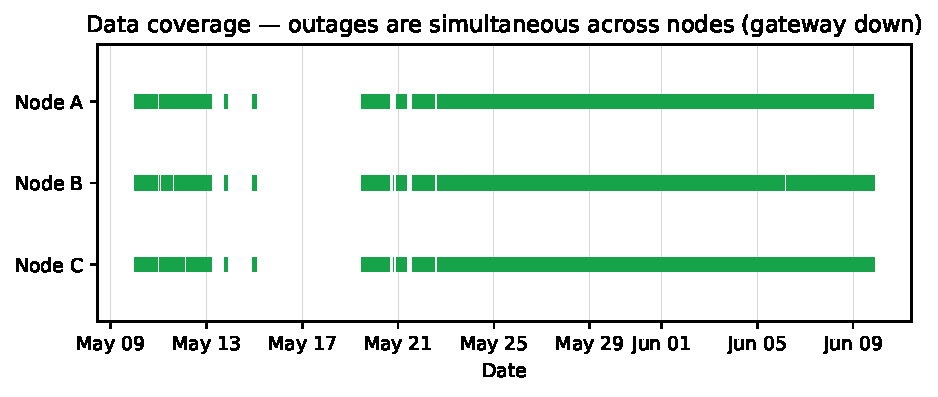
\includegraphics[width=0.9\linewidth]{val-cobertura.pdf}
\caption{Data coverage of the three nodes. Outages are simultaneous across nodes, corresponding to gateway-off periods rather than LoRa link failures.}
\label{fig:cobertura}
\end{figure}

\begin{figure}[h]\centering
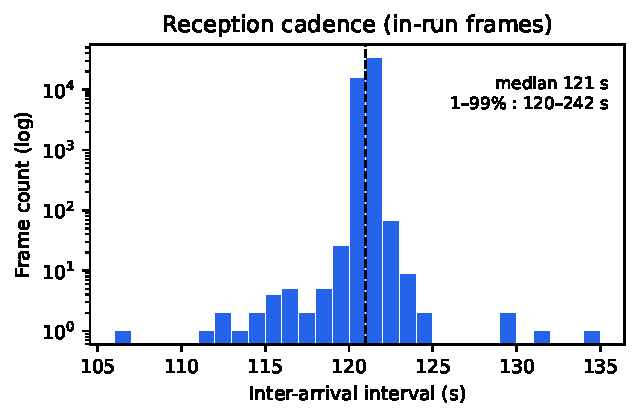
\includegraphics[width=0.6\linewidth]{val-intervalos.pdf}
\caption{Inter-arrival interval distribution during active intervals (log scale); most frames arrive near the 121~s median.}
\label{fig:intervalos}
\end{figure}

\textbf{Capabilities and limitations.}
\begin{itemize}[noitemsep]
\item Measures surface temperature with a three-wire PT100 over the MAX31865 range; per-node configurable offset.
\item LoRa link availability $>$97\% (active intervals) at a 121~s cadence over 32 days.
\item Local operation with per-sensor daily history (up to 30 days on-device) and no Internet dependency.
\item Temperature readings agreed with an infrared reference within $\pm$0.4~$^{\circ}$C; a strict $\leq$1~$^{\circ}$C validation requires a calibrated contact reference (planned).
\item Battery autonomy on the order of months (a 5-day discharge test gives $\approx$177 days conservatively and $\approx$10 months from the LiPo-curve model on a 1000~mAh cell; $\approx$0.13--0.24~mA average at a 1.9\% duty cycle), far exceeding typical requirements.
\item Limitations: absolute temperature accuracy depends on PT100 tolerance, mounting and per-node calibration; RSSI/SNR are not exposed by the current firmware; end-to-end latency was not measured (no node--gateway clock synchronization).
\end{itemize}

\FloatBarrier

\noindent
\textbf{Ethics statements}\\
This work did not involve human subjects or animal experiments.

\noindent
\textbf{CRediT author statement}\\
\textbf{Jesus Andre Bojaca Lopez}: Conceptualization, Methodology, Software, Investigation, Writing -- Original draft. \textbf{David Santiago Puentes Cardenas}: Conceptualization, Hardware, Software, Validation, Data curation, Writing -- Review \& Editing. \textbf{Jhon Edwin Vera}: Supervision. \textbf{Sergio Francisco Mora Martinez}: Supervision.

\noindent
\textbf{Acknowledgements}\\
The authors thank the partner company that provided access to the pilot plant. This research did not receive any specific grant from funding agencies in the public, commercial, or not-for-profit sectors.

\noindent
\textbf{References}\\
\begin{enumerate}[label={[\arabic*]}, noitemsep]
\item I. F. Akyildiz, W. Su, Y. Sankarasubramaniam, and E. Cayirci, ``Wireless sensor networks: A survey,'' \textit{Computer Networks}, vol. 38, no. 4, pp. 393--422, 2002.
\item J. Yick, B. Mukherjee, and D. Ghosal, ``Wireless sensor network survey,'' \textit{Computer Networks}, vol. 52, no. 12, pp. 2292--2330, 2008.
\item M. Centenaro, L. Vangelista, A. Zanella, and M. Zorzi, ``Long-range communications in unlicensed bands: the rising stars in the IoT and smart city scenarios,'' \textit{IEEE Wireless Communications}, vol. 23, no. 5, pp. 60--67, 2016.
\item A. K. S. Jardine, D. Lin, and D. Banjevic, ``A review on machinery diagnostics and prognostics implementing condition-based maintenance,'' \textit{Mechanical Systems and Signal Processing}, vol. 20, no. 7, pp. 1483--1510, 2006.
\item Advantech Co., Ltd., ``WISE-2410 LoRaWAN wireless condition monitoring sensor,'' Data Sheet, 2024.
\end{enumerate}

\end{document}
